\documentclass[../notes.tex]{subfiles}

\pagestyle{main}
\renewcommand{\chaptermark}[1]{\markboth{\chaptername\ \thechapter\ (#1)}{}}
\stepcounter{chapter}

\begin{document}




\chapter{X-Ray Diffraction}
\section{XRD Analysis 2}
\begin{itemize}
    \item \marginnote{1/10:}Dealing with broadening of the XRD beam.
    \begin{itemize}
        \item Synchrotron radiation gets you better resolution.
    \end{itemize}
    \item How do you get a cleaner spectra, given this one?
    \begin{figure}[h!]
        \centering
        \begin{tikzpicture}
            \draw (0,2) -- (0,0) -- (5,0);
    
            \draw [rex,thick] (0.1,0.7)
                to[out=-50,in=180,looseness=0.7] (0.7,0.5)
                to[out=0,in=180,out looseness=0.3,in looseness=0.05] (0.9,1.8)
                to[out=0,in=180,out looseness=0.05,in looseness=0.3] (1.1,0.45)
                to[bend right=15,looseness=0.4] (1.5,0.4)
                to[out=0,in=180,out looseness=0.3,in looseness=0.05] (1.6,1)
                to[out=0,in=180,out looseness=0.05,in looseness=0.3] (1.7,0.38)
                to[bend right=15,looseness=0.4] (2.5,0.35)
                to[out=0,in=180,out looseness=0.3,in looseness=0.05] (2.6,1.2)
                to[out=0,in=180,out looseness=0.05,in looseness=0.3] (2.7,0.35)
                to[out=0,in=180,out looseness=1.5,in looseness=0.3] (2.9,0.2)
                to (4.9,0.2)
            ;
        \end{tikzpicture}
        \caption{Enhancing XRD results.}
        \label{fig:enhanceXRD}
    \end{figure}
    \begin{itemize}
        \item In general:
        \begin{itemize}
            \item You can change divergence slits, filter, and masks.
            \item You can't change the monochromator, however, because it's built into the machine.
        \end{itemize}
        \item In this particular case:
        \begin{itemize}
            \item The issue is the high background which may be covering up smaller peaks.
            \item Solution: Use a smaller divergence slit and more masks.
            \item Another problem that could be causing high background is X-ray fluorescence, so check to make sure that your sample doesn't have iron or other similar things contaminating it.
        \end{itemize}
    \end{itemize}
    \item The principle of Bragg's law.
    \begin{itemize}
        \item The Braggs proposed that crystals can be described in terms of layers or planes of atoms.
        \item Their theoretical planes behave like \textbf{reflecting planes}.
        \item Strong "reflected" beams are produced when the path differences between reflections from successive planes in a family is equal to a whole number of wavelengths.
        \begin{itemize}
            \item If we want to see something, neighboring planes' waves must be in phase, interfering constructively to amplify their intensity rather than dampening it with destructive interference.
        \end{itemize}
        \item This approach is not correct in a physical sense --- planes do not reflect X-rays. However, it is correct in a geometrical sense and provides us with a very simple expression for the analysis of crystal structure.
    \end{itemize}
    \item \textbf{Reflecting plane}: A plane for which the angle of incidence equals the angle of reflection.
    \item Conditions that are necessary to make the phases of the beams coincide.
    \begin{itemize}
        \item Refer to Figure \ref{fig:BraggDeriv} throughout the following.
        \item The angles of the incident and "reflected" photons are equal.
        \item The rays of the incident are always in phase and are parallel up to the point at which the top beam reaches the top layer at atom $O$.
        \item The second beam continues to the next layer where it is scattered at atom $B$. If the two beams travel in adjacent and parallel fashion, the beam scattered at atom $B$ travels an extra distance $AB+BC$. This extra distance should be equal to a whole number of wavelengths.
        \item Again, a diffracted beam \emph{looks} reflected, but what it really is is scattered radiation. Drill home that planes are not physically accurate!
    \end{itemize}
    \item How to derive the Bragg's Law formula.
    \begin{figure}[h!]
        \centering
        \begin{tikzpicture}[
            every node/.style={black}
        ]
            \footnotesize
            \draw (0,-3.5) -- (0,2.5);
            \draw [dash pattern=on 2pt off 1pt]
                foreach \y in {0,-1.5,-3} {
                    (-2.5,\y) -- (2.5,\y)
                }
            ;
    
            \coordinate (1) at (-1,0);
            \coordinate (B) at (0,-1.5);
            \coordinate (2) at (1,0);
            \coordinate (O) at (0,0);
            \draw [help lines] ($(1)!-0.9!(B)$) -- (B) -- ($(B)!1.9!(2)$);
            \draw [help lines] ($(O)!-1.4!(1,-1.5)$) -- (O) -- ($(O)!1.4!(1,1.5)$);
            \draw [blx,very thick,-latex] ($(1)!-0.9!(B)$) -- ($(1)!-0.4!(B)$);
            \draw [blx,very thick,-latex] ($(O)!-1.4!(1,-1.5)$) -- ($(O)!-0.9!(1,-1.5)$);
            \draw [blx,very thick,-latex] ($(B)!1.4!(2)$) -- ($(B)!1.9!(2)$);
            \draw [blx,very thick,-latex] ($(O)!0.9!(1,1.5)$) -- ($(O)!1.4!(1,1.5)$);
            \draw [blx,semithick,<->,shorten <=1pt,shorten >=1pt] (2.3,0) -- node[left]{$d$} (2.3,-1.5);
    
            \coordinate (A) at ({-9/13},{-6/13});
            \coordinate (C) at ({9/13},{-6/13});
            \draw [rex,very thick] (A) node[left]{$A$} -- (B) node[below=1.5mm,fill=white,inner sep=2pt]{$B$} -- (C) node[right]{$C$};
            \draw [rex,very thick,dashed] (A) -- (O) -- (C);
    
            \coordinate (3) at (-2,0);
            \coordinate (3a) at ($(1)!-0.9!(B)$);
            \coordinate (Oa) at ($(O)!-1.4!(1,-1.5)$);
            \pic [draw=grx,semithick,pic text={$\alpha$},angle radius=4mm,angle eccentricity=0.7] {angle=1--O--A};
            \pic [draw=blx,semithick,pic text={$\theta$},angle radius=4mm,angle eccentricity=0.7] {angle=A--1--O};
            \pic [draw=blx,semithick,pic text={$\theta$},angle radius=4mm,angle eccentricity=0.7] {angle=3a--1--3};
            \pic [draw=blx,semithick,pic text={$\theta$},angle radius=4mm,angle eccentricity=0.7] {angle=Oa--O--1};
            \pic [draw=rex,semithick,pic text={$x$},angle radius=4mm,angle eccentricity=0.7] {angle=A--O--B};
    
            \foreach \x in {-2,...,2} {
                \foreach \y in {-3,-1.5,0} {
                    \fill [orx] (\x,\y) circle (1.5mm);
                }
            }
        \end{tikzpicture}
        \caption{Bragg's Law derivation.}
        \label{fig:BraggDeriv}
    \end{figure}
    \begin{itemize}
        \item Since $\theta+\alpha=\ang{90}$ and $\theta+x=\ang{90}$, we know that
        \begin{equation*}
            x = \theta
        \end{equation*}
        \item This combined with the observation that $\sin(x)=AB/d$ implies that
        \begin{align*}
            \sin\theta &= \frac{AB}{d}\\
            AB &= d\sin\theta
        \end{align*}
        \item Lastly, we may observe that $AB=BC$. Therefore, the total phase shift is
        \begin{equation*}
            2AB = 2d\sin\theta
        \end{equation*}
        \item Since we require that this is a whole number of wavelengths, our final condition is
        \begin{equation*}
            n\lambda = 2d\sin\theta
        \end{equation*}
        where $n$ is an integer determined by the order given, $\lambda$ is the wavelength of the X-rays, $d$ is the spacing between the planes in the atomic lattice, and $\theta$ is the angle between the incident ray and the scattering planes.
        \begin{itemize}
            \item This condition is called \textbf{Bragg's Law}.
        \end{itemize}
        \item Note that copper's $\lambda=\SI{1.54}{\angstrom}$ is the most common wavelength with which to work.
    \end{itemize}
    \item Mineralogy --- Inspiration for crystallography.
    \begin{itemize}
        \item Happened way before all of this math, when scientists had far fewer tools.
        \item Researchers could only observe a crystal's \textbf{habit} and cleavage planes, and measure interfacial angles with a \textbf{goniometer}.
        \item Ren\'{e} Just Ha\"{u}y postulates in 1801: Crystal structures are made up of orderly arrangements of integrant molecules in successive layers, according to geometrical laws of crystallization.
        \item Ha\"{u}y formulated the \textbf{theory of the rational indices} of the faces of a crystal, which is important for crystallographic calculations.
        \item By 1792, he had identified several parallelepipeds to explain shapes of a few crystals.
        \item This work, which may now seem elementary, is extremely impressive since he had so few tools.
    \end{itemize}
    \item \textbf{Habit}: The tendency for specimens of a mineral to repeatedly grow into characteristic shapes.
    \item \textbf{Goniometer}: An instrument that either measures an angle or allows an object to be rotated to a precise angular position.
    \item \textbf{Theory of rational indices}: The theory that the intercepts of a crystal face with the crystallographic axes can be expressed as $a/h$, $b/k$, and $c/l$, where $1/h$, $1/k$, and $1/l$ are three simple rational numbers.
    \item Type of Lattice Systems.
    \begin{itemize}
        \item Ha\"{u}y (1784): The periodicity of crystalline materials involves the basic repetition of a basic unit called the \textbf{unit cell}.
        \item Crystalline materials are formed by the repetition in (2D, 3D, etc.) space of cells (or \textbf{crystallites}).
        \item In 3D space, cells are defined by three non-coplanar vectors (called \textbf{fundamental translations}).
        \item There are 7 types of cells that together cover all possible point lattices.
        \item Important: Crystal structures are defined by a \textbf{basis} and a \textbf{lattice}.
    \end{itemize}
    \item \textbf{Basis}: \emph{What} gets repeated in the crystal structure.
    \item \textbf{Lattice}: \emph{How} it gets repeated.
    \item Bravais lattices.
    \begin{figure}[h!]
        \centering
        \includegraphics[width=0.45\linewidth]{BravaisTF.png}
        \caption{Decomposition of a crystal into its Bravais lattice.}
        \label{fig:BravaisTF}
    \end{figure}
    \begin{itemize}
        \item Auguste Bravais (1848) found mathematically that the number of crystalline lattices is finite.
        \item It is a fully geometrical concept and has nothing to do with atoms or crystalline planes.
        \item Bravais lattices are the basic lattice arrangements. All other lattices can simplify into one of the Bravais lattices. Bravais lattices move a \emph{specific} basis by a translation.
        \item There are 14 3D Bravais lattices.
        \item Bravais lattices only take into account \emph{translational} symmetry (this is important!).
        \item If you can exactly repeat the entire structure by a set of translations, that is the Bravais lattice.
        \item Other symmetries, like reflection or inversion, are captured in point groups and space groups, not by Bravais lattices.
    \end{itemize}
    \item 1D Bravais lattice.
    \begin{figure}[h!]
        \centering
        \begin{tikzpicture}
            \draw [dashed]
                (-5.25,0) -- (-6.5,0)
                (5.25,0) -- (6.5,0)
            ;
            \draw (-5.25,0) -- (5.25,0);
    
            \fill [fill=grx] ({-2.8-2.45},0) circle (1.5mm);
            \fill [fill=blx] ({-2.8-2.15},0) circle (0.7mm);
            \fill [fill=rex] ({-2.8-1.8},0) circle (1mm);
            % 
            \fill [fill=rex] ({-2.8-1.05},0) circle (1mm);
            \fill [fill=blx] ({-2.8-0.75},0) circle (0.7mm);
            \fill [fill=grx] ({-2.8-0.4},0) circle (1.5mm);
            % 
            \fill [fill=grx] (-2.45,0) circle (1.5mm);
            \fill [fill=blx] (-2.15,0) circle (0.7mm);
            \fill [fill=rex] (-1.8,0) circle (1mm);
            % 
            \fill [fill=rex] (-1.05,0) circle (1mm);
            \fill [fill=blx] (-0.75,0) circle (0.7mm);
            \fill [fill=grx] (-0.4,0) circle (1.5mm);
            % 
            \fill [fill=grx] (0.4,0) circle (1.5mm);
            \fill [fill=blx] (0.75,0) circle (0.7mm);
            \fill [fill=rex] (1.05,0) circle (1mm);
            % 
            \fill [fill=rex] (1.8,0) circle (1mm);
            \fill [fill=blx] (2.15,0) circle (0.7mm);
            \fill [fill=grx] (2.45,0) circle (1.5mm);
            % 
            \fill [fill=grx] ({2.85+0.4},0) circle (1.5mm);
            \fill [fill=blx] ({2.85+0.75},0) circle (0.7mm);
            \fill [fill=rex] ({2.85+1.05},0) circle (1mm);
            % 
            \fill [fill=rex] ({2.85+1.8},0) circle (1mm);
            \fill [fill=blx] ({2.85+2.15},0) circle (0.7mm);
            \fill [fill=grx] ({2.85+2.45},0) circle (1.5mm);
    
            \draw [|-|] (-5.65,0.5) -- node[above]{${\color{rex}X}$} (-4.25,0.5);
            \draw [|-|] (-5.65,-0.5) -- node[below]{${\color{grx}\checkmark}$} (-2.8,-0.5);
        \end{tikzpicture}
        \caption{1D Bravais lattices.}
        \label{fig:Bravais1D}
    \end{figure}
    \begin{itemize}
        \item Only one vector, hence only one possible Bravais lattice.
        \item Bravais lattices do not allow mirror symmetry, only translation. Thus, we must choose as our basis the smallest structure that repeats \emph{translationally}.
    \end{itemize}
    \item 2D Bravais lattice.
    \begin{figure}[h!]
        \centering
        \begin{subfigure}[b]{0.4\linewidth}
            \centering
            \includegraphics[width=0.9\linewidth]{Bravais2Da.png}
            \caption{Centered cubic?}
            \label{fig:Bravais2Da}
        \end{subfigure}
        \begin{subfigure}[b]{0.4\linewidth}
            \centering
            \includegraphics[width=0.7\linewidth]{Bravais2Db.png}
            \caption{Hexagonal?}
            \label{fig:Bravais2Db}
        \end{subfigure}
        \caption{2D Bravais lattices.}
        \label{fig:Bravais2D}
    \end{figure}
    \begin{itemize}
        \item There are five 2D Bravais lattices.
        \begin{enumerate}
            \item Square ($a=b$, $\theta=\ang{90}$).
            \item Hexagonal ($a=b$, $\theta=\ang{120}$).
            \item Rectangular ($a\neq b$, $\theta=\ang{90}$).
            \item Centered rectangular (see below).
            \item Rhomboidal ($a\neq b$, $\theta\neq\ang{90}$).
        \end{enumerate}
        \item Rhomboidal is also known as \textbf{oblique}.
        \item There does exist centered rectangular (a rectangular lattice with an additional vertex in the center of each rectangle), but there does not exist "centered cubic" because a smaller, rotated square can represent the entire lattice, so "centered cubic" is really just square. See Figure \ref{fig:Bravais2Da}.
        \item The "hexagonal" Bravais lattice can be simplified into a rhombus, but hexagon shows "true" symmetry (i.e., rotation, inversion, etc.). See Figure \ref{fig:Bravais2Db}.
        \item The honeycomb is not a Bravais lattice. Why??
    \end{itemize}
    \item 3D Bravais lattice.
    % \item Triclinic systems.
    % \begin{itemize}
    %     \item $a\neq b\neq c$, $\alpha\neq\beta\neq\gamma\neq\ang{90}$.
    %     \item 1 possible type of Bravais lattice.
    % \end{itemize}
    % \item Monoclinic system.
    % \begin{itemize}
    %     \item ...
    % \end{itemize}
    % \item Orthorhobmic system.
    % \begin{itemize}
    %     \item ...
    % \end{itemize}
    % \item Tetragonal system.
    % \begin{itemize}
    %     \item ...
    % \end{itemize}
    % \item Rhombohedral system.
    % \begin{itemize}
    %     \item ...
    % \end{itemize}
    % \item Hexagonal system.
    % \begin{itemize}
    %     \item ...
    % \end{itemize}
    % \item Cubic system.
    % \begin{itemize}
    %     \item ...
    % \end{itemize}
    \begin{table}[H]
        \centering
        \small
        \renewcommand{\arraystretch}{1.4}
        \begin{tabular}{ccccc}
             & P & I & C & F\\
            \begin{tabular}{@{}c@{}}
                Triclinic\\[-2mm]
                \footnotesize
                $a\neq b\neq c$\\[-2mm]
                \footnotesize
                $\alpha\neq\beta\neq\gamma\neq\ang{90}$
            \end{tabular}
                & \tikz[baseline={(0,0.6)},scale=0.7]{
                    \path (0,-0.4) -- (0,2.3);
                    \filldraw [fill=white]
                        (0,0) coordinate (O) circle (1.5pt)
                        (1.38,0) coordinate (a) circle (1.5pt)
                        (0.64,0.26) coordinate (b) circle (1.5pt)
                        (-0.22,1.6) coordinate (c) circle (1.5pt)
                        ($(a)+(b)$) coordinate (ab) circle (1.5pt)
                        ($(a)+(c)$) coordinate (ac) circle (1.5pt)
                        ($(b)+(c)$) coordinate (bc) circle (1.5pt)
                        ($(a)+(b)+(c)$) coordinate (abc) circle (1.5pt)
                    ;
                    \begin{scope}[on background layer]
                        \draw [line join=bevel]
                            (O) -- (a) -- (ab) -- (b) -- cycle
                            (c) -- (ac) -- (abc) -- (bc) -- cycle
                            (O) -- (c)
                            (a) -- (ac)
                            (b) -- (bc)
                            (ab) -- (abc)
                        ;
                    \end{scope}
                }
                &  &  & \\
            \begin{tabular}{@{}c@{}}
                Monoclinic\\[-2mm]
                \footnotesize
                $a\neq b\neq c$\\[-2mm]
                \footnotesize
                $\beta=\gamma=\ang{90}$\\[-2mm]
                \footnotesize
                $\alpha\neq\ang{90}$
            \end{tabular}
                & \tikz[baseline={(0,0.6)},scale=0.7]{
                    \path (0,-0.4) -- (0,2.3);
                    \filldraw [fill=white]
                        (0,0) coordinate (O) circle (1.5pt)
                        (1.3,0) coordinate (a) circle (1.5pt)
                        (0.62,0.24) coordinate (b) circle (1.5pt)
                        (0,1.65) coordinate (c) circle (1.5pt)
                        ($(a)+(b)$) coordinate (ab) circle (1.5pt)
                        ($(a)+(c)$) coordinate (ac) circle (1.5pt)
                        ($(b)+(c)$) coordinate (bc) circle (1.5pt)
                        ($(a)+(b)+(c)$) coordinate (abc) circle (1.5pt)
                    ;
                    \begin{scope}[on background layer]
                        \draw [line join=bevel]
                            (O) -- (a) -- (ab) -- (b) -- cycle
                            (c) -- (ac) -- (abc) -- (bc) -- cycle
                            (O) -- (c)
                            (a) -- (ac)
                            (b) -- (bc)
                            (ab) -- (abc)
                        ;
                    \end{scope}
                }
                & \tikz[baseline={(0,0.6)},scale=0.7]{
                    \path (0,-0.4) -- (0,2.3);
                    \filldraw [fill=white]
                        (0,0) coordinate (O) circle (1.5pt)
                        (1.3,0) coordinate (a) circle (1.5pt)
                        (0.62,0.24) coordinate (b) circle (1.5pt)
                        (0,1.65) coordinate (c) circle (1.5pt)
                        ($(a)+(b)$) coordinate (ab) circle (1.5pt)
                        ($(a)+(c)$) coordinate (ac) circle (1.5pt)
                        ($(b)+(c)$) coordinate (bc) circle (1.5pt)
                        ($(a)+(b)+(c)$) coordinate (abc) circle (1.5pt)
                        ($0.5*($(a)+(b)+(c)$)$)circle (1.5pt)
                    ;
                    \begin{scope}[on background layer]
                        \draw [line join=bevel]
                            (O) -- (a) -- (ab) -- (b) -- cycle
                            (c) -- (ac) -- (abc) -- (bc) -- cycle
                            (O) -- (c)
                            (a) -- (ac)
                            (b) -- (bc)
                            (ab) -- (abc)
                        ;
                        \draw [dash pattern=on 2pt off 2pt] (bc) -- (a);
                    \end{scope}
                }
                &  & \\
            \begin{tabular}{@{}c@{}}
                Orthorhombic\\[-2mm]
                \footnotesize
                $a\neq b\neq c$\\[-2mm]
                \footnotesize
                $\alpha=\beta=\gamma=\ang{90}$
            \end{tabular}
                & \tikz[baseline={(0,0.6)},scale=0.7]{
                    \path (0,-0.4) -- (0,2.4);
                    \filldraw [fill=white]
                        (0,0) coordinate (O) circle (1.5pt)
                        (1.38,0) coordinate (a) circle (1.5pt)
                        (0.27,0.21) coordinate (b) circle (1.5pt)
                        (0,1.78) coordinate (c) circle (1.5pt)
                        ($(a)+(b)$) coordinate (ab) circle (1.5pt)
                        ($(a)+(c)$) coordinate (ac) circle (1.5pt)
                        ($(b)+(c)$) coordinate (bc) circle (1.5pt)
                        ($(a)+(b)+(c)$) coordinate (abc) circle (1.5pt)
                    ;
                    \begin{scope}[on background layer]
                        \draw [line join=bevel]
                            (O) -- (a) -- (ab) -- (b) -- cycle
                            (c) -- (ac) -- (abc) -- (bc) -- cycle
                            (O) -- (c)
                            (a) -- (ac)
                            (b) -- (bc)
                            (ab) -- (abc)
                        ;
                    \end{scope}
                }
                & \tikz[baseline={(0,0.6)},scale=0.7]{
                    \path (0,-0.4) -- (0,2.4);
                    \filldraw [fill=white]
                        (0,0) coordinate (O) circle (1.5pt)
                        (1.38,0) coordinate (a) circle (1.5pt)
                        (0.27,0.21) coordinate (b) circle (1.5pt)
                        (0,1.78) coordinate (c) circle (1.5pt)
                        ($(a)+(b)$) coordinate (ab) circle (1.5pt)
                        ($(a)+(c)$) coordinate (ac) circle (1.5pt)
                        ($(b)+(c)$) coordinate (bc) circle (1.5pt)
                        ($(a)+(b)+(c)$) coordinate (abc) circle (1.5pt)
                        ($0.5*($(a)+(b)+(c)$)$)circle (1.5pt)
                    ;
                    \begin{scope}[on background layer]
                        \draw [line join=bevel]
                            (O) -- (a) -- (ab) -- (b) -- cycle
                            (c) -- (ac) -- (abc) -- (bc) -- cycle
                            (O) -- (c)
                            (a) -- (ac)
                            (b) -- (bc)
                            (ab) -- (abc)
                        ;
                        \draw [dash pattern=on 2pt off 2pt] (bc) -- (a);
                    \end{scope}
                }
                & \tikz[baseline={(0,0.6)},scale=0.7]{
                    \path (0,-0.4) -- (0,2.4);
                    \filldraw [fill=white]
                        (0,0) coordinate (O) circle (1.5pt)
                        (1.38,0) coordinate (a) circle (1.5pt)
                        (0.27,0.21) coordinate (b) circle (1.5pt)
                        (0,1.78) coordinate (c) circle (1.5pt)
                        ($(a)+(b)$) coordinate (ab) circle (1.5pt)
                        ($(a)+(c)$) coordinate (ac) circle (1.5pt)
                        ($(b)+(c)$) coordinate (bc) circle (1.5pt)
                        ($(a)+(b)+(c)$) coordinate (abc) circle (1.5pt)
                        ($0.5*($(a)+(b)$)$)circle (1.5pt)
                        ($0.5*($(a)+(b)$)+(c)$)circle (1.5pt)
                    ;
                    \begin{scope}[on background layer]
                        \draw [line join=bevel]
                            (O) -- (a) -- (ab) -- (b) -- cycle
                            (c) -- (ac) -- (abc) -- (bc) -- cycle
                            (O) -- (c)
                            (a) -- (ac)
                            (b) -- (bc)
                            (ab) -- (abc)
                        ;
                    \end{scope}
                }
                & \tikz[baseline={(0,0.6)},scale=0.7]{
                    \path (0,-0.4) -- (0,2.4);
                    \filldraw [fill=white]
                        (0,0) coordinate (O) circle (1.5pt)
                        (1.38,0) coordinate (a) circle (1.5pt)
                        (0.27,0.21) coordinate (b) circle (1.5pt)
                        (0,1.78) coordinate (c) circle (1.5pt)
                        ($(a)+(b)$) coordinate (ab) circle (1.5pt)
                        ($(a)+(c)$) coordinate (ac) circle (1.5pt)
                        ($(b)+(c)$) coordinate (bc) circle (1.5pt)
                        ($(a)+(b)+(c)$) coordinate (abc) circle (1.5pt)
                        ($0.5*($(a)+(b)$)$)circle (1.5pt)
                        ($0.5*($(a)+(b)$)+(c)$)circle (1.5pt)
                        ($0.5*($(a)+(c)$)$)circle (1.5pt)
                        ($0.5*($(a)+(c)$)+(b)$)circle (1.5pt)
                        ($0.5*($(b)+(c)$)$)circle (1.5pt)
                        ($0.5*($(b)+(c)$)+(a)$)circle (1.5pt)
                    ;
                    \begin{scope}[on background layer]
                        \draw [line join=bevel]
                            (O) -- (a) -- (ab) -- (b) -- cycle
                            (c) -- (ac) -- (abc) -- (bc) -- cycle
                            (O) -- (c)
                            (a) -- (ac)
                            (b) -- (bc)
                            (ab) -- (abc)
                        ;
                    \end{scope}
                }
                \\
            \begin{tabular}{@{}c@{}}
                Tetragonal\\[-2mm]
                \footnotesize
                $a=b\neq c$\\[-2mm]
                \footnotesize
                $\alpha=\beta=\gamma=\ang{90}$
            \end{tabular}
            & \tikz[baseline={(0,0.6)},scale=0.7]{
                \path (0,-0.4) -- (0,2.4);
                \filldraw [fill=white]
                    (0,0) coordinate (O) circle (1.5pt)
                    (1.38,0) coordinate (a) circle (1.5pt)
                    (0.37,0.21) coordinate (b) circle (1.5pt)
                    (0,1.78) coordinate (c) circle (1.5pt)
                    ($(a)+(b)$) coordinate (ab) circle (1.5pt)
                    ($(a)+(c)$) coordinate (ac) circle (1.5pt)
                    ($(b)+(c)$) coordinate (bc) circle (1.5pt)
                    ($(a)+(b)+(c)$) coordinate (abc) circle (1.5pt)
                ;
                \begin{scope}[on background layer]
                    \draw [line join=bevel]
                        (O) -- (a) -- (ab) -- (b) -- cycle
                        (c) -- (ac) -- (abc) -- (bc) -- cycle
                        (O) -- (c)
                        (a) -- (ac)
                        (b) -- (bc)
                        (ab) -- (abc)
                    ;
                \end{scope}
            }
            & \tikz[baseline={(0,0.6)},scale=0.7]{
                \path (0,-0.4) -- (0,2.4);
                \filldraw [fill=white]
                    (0,0) coordinate (O) circle (1.5pt)
                    (1.38,0) coordinate (a) circle (1.5pt)
                    (0.37,0.21) coordinate (b) circle (1.5pt)
                    (0,1.78) coordinate (c) circle (1.5pt)
                    ($(a)+(b)$) coordinate (ab) circle (1.5pt)
                    ($(a)+(c)$) coordinate (ac) circle (1.5pt)
                    ($(b)+(c)$) coordinate (bc) circle (1.5pt)
                    ($(a)+(b)+(c)$) coordinate (abc) circle (1.5pt)
                    ($0.5*($(a)+(b)+(c)$)$)circle (1.5pt)
                ;
                \begin{scope}[on background layer]
                    \draw [line join=bevel]
                        (O) -- (a) -- (ab) -- (b) -- cycle
                        (c) -- (ac) -- (abc) -- (bc) -- cycle
                        (O) -- (c)
                        (a) -- (ac)
                        (b) -- (bc)
                        (ab) -- (abc)
                    ;
                    \draw [dash pattern=on 2pt off 2pt] (bc) -- (a);
                \end{scope}
            }
                &  & \\
            \begin{tabular}{@{}c@{}}
                Rhombohedral\\[-2mm]
                \footnotesize
                $a=b=c$\\[-2mm]
                \footnotesize
                $\alpha=\beta=\gamma\neq\ang{90}$
            \end{tabular}
                & \tikz[baseline={(0,0.9)},scale=0.7]{
                    \path (0,-0.4) -- (0,2.4);
                    \filldraw [fill=white]
                        (0,0) coordinate (O) circle (1.5pt)
                        (1.3,0.23) coordinate (a) circle (1.5pt)
                        (0.62,0.41) coordinate (b) circle (1.5pt)
                        (0.79,1.33) coordinate (c) circle (1.5pt)
                        ($(a)+(b)$) coordinate (ab) circle (1.5pt)
                        ($(a)+(c)$) coordinate (ac) circle (1.5pt)
                        ($(b)+(c)$) coordinate (bc) circle (1.5pt)
                        ($(a)+(b)+(c)$) coordinate (abc) circle (1.5pt)
                    ;
                    \begin{scope}[on background layer]
                        \draw [line join=bevel]
                            (O) -- (a) -- (ab) -- (b) -- cycle
                            (c) -- (ac) -- (abc) -- (bc) -- cycle
                            (O) -- (c)
                            (a) -- (ac)
                            (b) -- (bc)
                            (ab) -- (abc)
                        ;
                    \end{scope}
                }
                &  &  & \\
            \begin{tabular}{@{}c@{}}
                Hexagonal\\[-2mm]
                \footnotesize
                $a=b\neq c$\\[-2mm]
                \footnotesize
                $\alpha=\beta=\ang{90}$\\[-2mm]
                \footnotesize
                $\gamma=\ang{120}$
            \end{tabular}
                & \tikz[baseline={(0,0.7)},scale=0.7]{
                    \path (0,-0.4) -- (0,2.5);
                    \filldraw [fill=white]
                        (0,0) coordinate (O) circle (1.5pt)
                        (1.1,0) coordinate (a) circle (1.5pt)
                        (-0.79,0.23) coordinate (b) circle (1.5pt)
                        (0,1.81) coordinate (c) circle (1.5pt)
                        ($(a)+(b)$) coordinate (ab) circle (1.5pt)
                        ($(a)+(c)$) coordinate (ac) circle (1.5pt)
                        ($(b)+(c)$) coordinate (bc) circle (1.5pt)
                        ($(a)+(b)+(c)$) coordinate (abc) circle (1.5pt)
                    ;
                    \begin{scope}[on background layer]
                        \draw [line join=bevel]
                            (O) -- (a) -- (ab) -- (b) -- cycle
                            (c) -- (ac) -- (abc) -- (bc) -- cycle
                            (O) -- (c)
                            (a) -- (ac)
                            (b) -- (bc)
                            (ab) -- (abc)
                        ;
                    \end{scope}
                }
                &  &  & \\
            \begin{tabular}{@{}c@{}}
                Cubic\\[-2mm]
                \footnotesize
                $a=b=c$\\[-2mm]
                \footnotesize
                $\alpha=\beta=\gamma=\ang{90}$
            \end{tabular}
                & \tikz[baseline={(0,0.6)},scale=0.7]{
                    \path (0,-0.5) -- (0,2.4);
                    \filldraw [fill=white]
                        (0,0) coordinate (O) circle (1.5pt)
                        (1.46,-0.06) coordinate (a) circle (1.5pt)
                        (0.42,0.34) coordinate (b) circle (1.5pt)
                        (0,1.63) coordinate (c) circle (1.5pt)
                        ($(a)+(b)$) coordinate (ab) circle (1.5pt)
                        ($(a)+(c)$) coordinate (ac) circle (1.5pt)
                        ($(b)+(c)$) coordinate (bc) circle (1.5pt)
                        ($(a)+(b)+(c)$) coordinate (abc) circle (1.5pt)
                    ;
                    \begin{scope}[on background layer]
                        \draw [line join=bevel]
                            (O) -- (a) -- (ab) -- (b) -- cycle
                            (c) -- (ac) -- (abc) -- (bc) -- cycle
                            (O) -- (c)
                            (a) -- (ac)
                            (b) -- (bc)
                            (ab) -- (abc)
                        ;
                    \end{scope}
                }
                & \tikz[baseline={(0,0.6)},scale=0.7]{
                    \path (0,-0.5) -- (0,2.4);
                    \filldraw [fill=white]
                        (0,0) coordinate (O) circle (1.5pt)
                        (1.46,-0.06) coordinate (a) circle (1.5pt)
                        (0.42,0.34) coordinate (b) circle (1.5pt)
                        (0,1.63) coordinate (c) circle (1.5pt)
                        ($(a)+(b)$) coordinate (ab) circle (1.5pt)
                        ($(a)+(c)$) coordinate (ac) circle (1.5pt)
                        ($(b)+(c)$) coordinate (bc) circle (1.5pt)
                        ($(a)+(b)+(c)$) coordinate (abc) circle (1.5pt)
                        ($0.5*($(a)+(b)+(c)$)$)circle (1.5pt)
                    ;
                    \begin{scope}[on background layer]
                        \draw [line join=bevel]
                            (O) -- (a) -- (ab) -- (b) -- cycle
                            (c) -- (ac) -- (abc) -- (bc) -- cycle
                            (O) -- (c)
                            (a) -- (ac)
                            (b) -- (bc)
                            (ab) -- (abc)
                        ;
                        \draw [dash pattern=on 2pt off 2pt] (bc) -- (a);
                    \end{scope}
                }
                & 
                & \tikz[baseline={(0,0.6)},scale=0.7]{
                    \path (0,-0.5) -- (0,2.4);
                    \filldraw [fill=white]
                        (0,0) coordinate (O) circle (1.5pt)
                        (1.46,-0.06) coordinate (a) circle (1.5pt)
                        (0.42,0.34) coordinate (b) circle (1.5pt)
                        (0,1.63) coordinate (c) circle (1.5pt)
                        ($(a)+(b)$) coordinate (ab) circle (1.5pt)
                        ($(a)+(c)$) coordinate (ac) circle (1.5pt)
                        ($(b)+(c)$) coordinate (bc) circle (1.5pt)
                        ($(a)+(b)+(c)$) coordinate (abc) circle (1.5pt)
                        ($0.5*($(a)+(b)$)$)circle (1.5pt)
                        ($0.5*($(a)+(b)$)+(c)$)circle (1.5pt)
                        ($0.5*($(a)+(c)$)$)circle (1.5pt)
                        ($0.5*($(a)+(c)$)+(b)$)circle (1.5pt)
                        ($0.5*($(b)+(c)$)$)circle (1.5pt)
                        ($0.5*($(b)+(c)$)+(a)$)circle (1.5pt)
                    ;
                    \begin{scope}[on background layer]
                        \draw [line join=bevel]
                            (O) -- (a) -- (ab) -- (b) -- cycle
                            (c) -- (ac) -- (abc) -- (bc) -- cycle
                            (O) -- (c)
                            (a) -- (ac)
                            (b) -- (bc)
                            (ab) -- (abc)
                        ;
                    \end{scope}
                }
                \\
        \end{tabular}
        \caption{Bravais lattices.}
        \label{tab:bravaisLattices}
    \end{table}
    \begin{itemize}
        \item Each lattice is a polyhedron.
        \begin{itemize}
            \item The polyhedrons can be described using three different vectors.
        \end{itemize}
        \item Some of the Bravais lattices can be expressed by other simple lattices: In 3D, the FCC lattice is also described by a rhombohedral lattice.
        \item There is no base-centered cubic Bravais lattice because what might be that is actually simple tetragonal.
    \end{itemize}
    \item There are 4 types of Bravais lattices.
    \begin{itemize}
        \item P - Primitive.
        \item I - Body centered.
        \item C - Base-centered.
        \item F - Face centered.
        \item More on these and how they correspond to space groups later.
    \end{itemize}
    \item \textbf{Unit cell}: The smallest group of atoms which has the overall symmetry of a crystal.
    \begin{itemize}
        \item Can be used to build the entire lattice by repetition in three dimensions.
        \item A 3D structure.
    \end{itemize}
    \item \textbf{Primitive cell}: The smallest possible element of a lattice.
    \begin{itemize}
        \item May or may not include all symmetry elements.
        \item Can have 2D or 3D structure.
    \end{itemize}
    \item Conventional and primitive cells.
    \begin{figure}[h!]
        \centering
        \begin{subfigure}[b]{0.33\linewidth}
            \centering
            \includegraphics[width=0.9\linewidth]{primitiveNonHexa.png}
            \caption{Primitive vs. non-primitive.}
            \label{fig:primitiveNonHexa}
        \end{subfigure}
        \begin{subfigure}[b]{0.32\linewidth}
            \centering
            \includegraphics[width=0.75\linewidth]{primitiveNonHexb.png}
            \caption{Simple hexagonal.}
            \label{fig:primitiveNonHexb}
        \end{subfigure}
        \begin{subfigure}[b]{0.33\linewidth}
            \centering
            \includegraphics[width=0.72\linewidth]{primitiveNonHexc.png}
            \caption{HCP.}
            \label{fig:primitiveNonHexc}
        \end{subfigure}
        \caption{Conventional vs. primitive cells.}
        \label{fig:primitiveNonHex}
    \end{figure}
    \begin{itemize}
        \item The hexagonal 2D Bravais lattice (the conventional cell) might also be described as rhombic (the primitive cell). See Figure \ref{fig:Bravais2Db}.
        \item The hexagonal 3D Bravais lattice is a hexagonal prism that can also be constructed from a primitive cell which is a parallelepiped.
        \item Know simple hexagonal vs. hexagonal close-packed (HCP). See Figures \ref{fig:primitiveNonHexb}-\ref{fig:primitiveNonHexc}.
        \item Clarification on primitive vs. non-primitive?? See Figure \ref{fig:primitiveNonHexa}.
        \item What is a lattice point??
    \end{itemize}
    \item Miller indices.
    \begin{itemize}
        \item In 1839, the British mineralogist William H. Miller used \emph{reciprocal quantities} --- namely, the integer numbers $h,k,l$ --- to describe crystal faces.
        \item Miller indices are used to specify directions and planes.
        \item These directions and planes could be in lattices or in crystals.
        \item Notation (important information!):
        \begin{itemize}
            \item $(h,k,l)$ represents a \textbf{point} (commas are used).
            \item $[hkl]$ represents a \textbf{direction}.
            \item $<hkl>$ represents a \textbf{family of directions}.
            \item $(hkl)$ represents a \textbf{plane}.
            \item $\{hkl\}$ represents a \textbf{family of planes}.
        \end{itemize}
        \item Be careful when writing/reading research literature to use/interpret the write notation.
        \item Negative numbers and directions are depicted with a bar on top of the number.
    \end{itemize}
    \item Miller indices for directions.
    \begin{itemize}
        \item Let's consider a 2D lattice with Miller indices $(4,-2)$.
        \begin{itemize}
            \item Defines a vector pointing in the direction $4\vec{a}-2\vec{b}$. It is parallel to many other vectors.
            \item The index $(4,-2)$ [notational issue here??] represents the set of all such parallel vectors.
        \end{itemize}
        \item The number of indices matches the dimension of lattice (e.g., 1D lattice has 1 Miller index, 2D lattice has 2 Miller indices, etc.).
        \item Fractions in $(r_1r_2r_3)$ are eliminated by multiplying all components by their common denominator. Example: $(1,3/4,1/2)$ will be expressed as $(4,3,2)$.
    \end{itemize}
    \item Miller indices: $hkl$ review.
    \begin{itemize}
        \item See \textcite{bib:CHEM26300Notes} for more.
        \item You just have to remember that Miller indices represent the reciprocals of the fractional intercepts which the plane makes with crystallographic axes.
        \item Notice how $(421)$ [i.e., parentheses] is used to denote a plane!
    \end{itemize}
    \item How to find Miller indices for planes.
    \begin{itemize}
        \item Great slide in the slideshow; one stop shop for Miller indices.
        \item The planes we will most commonly study are $(100)$, $(001)$, and $(010)$ planes.
        \item Algorithm.
        \begin{itemize}
            \item Identity the plane intercepts on the $x$-, $y$-, and $z$-axes.
            \item Define intercepts in fractional coordinates.
            \item Take the reciprocals of the fractional intercepts.
        \end{itemize}
    \end{itemize}
    \item Miller indices.
    \begin{itemize}
        \item Continuation of the previous slide but for slanted planes.
        \item Keep in mind that different planes have different chemical distributions. One plane in an oxide may be mostly oxygen; another may be mostly copper.
    \end{itemize}
    \item Crystal structure, lattice, etc.
    \begin{itemize}
        \item Crystal structure combines \textbf{lattice} with the \textbf{basis} again.
        \item A lattice is not a crystal. However, if the basis consists of one atom, crystal structures look exactly like the Bravais lattice.
        \item Common metallic crystal structures: BCC, FCC, hexagonal close-packed (HCP).
    \end{itemize}
    \item Example 1: Diamond.
    \begin{figure}[h!]
        \centering
        \includegraphics[width=0.2\linewidth]{structDiamond.png}
        \caption{Diamond crystal structure.}
        \label{fig:structDiamond}
    \end{figure}
    \begin{itemize}
        \item Bravais lattice: FCC with a two-atom basis.
        \item Crystal structure: Cubic diamond.
        \item Two atom basis at $(0,0,0)$ and $(1/4,1/4,1/4)$.
    \end{itemize}
    \item Example 2: \ce{NaCl}.
    \begin{itemize}
        \item Bravais lattice: FCC.
        \item Crystal structure: FCC.
        \item Both atoms make FCC lattices and you get the overall structure by inserting one lattice into the other.
    \end{itemize}
    \item Example 3: Primitive cubic substances.
    \begin{itemize}
        \item Examples: \ce{Fe}, \ce{CsCl}, and \ce{NiAl}.
        \item Bravais lattice: Primitive cubic with a two-atom basis (\ce{Cs} at $(0,0,0)$ and \ce{Cl} at $(1/2,1/2,1/2)$).
        \item Crystal structure: Primitive.
    \end{itemize}
    \item From Bravais lattices to a full description of crystalline structure.
    \begin{itemize}
        \item Bravais lattices: There are 14 and they account for translational symmetry. But there are also additional symmetry elements (rotation, inversion, reflection).
        \begin{itemize}
            \item We discount additional potential translation symmetry operations for now.
        \end{itemize}
        \item If you apply all of these other operations to the Bravais lattices, you get 32 crystal classes/point groups.
        \item If you add in \textbf{screw} and \textbf{glide} operations, you get 230 total space groups. This number does depend on the dimension of the space, though, i.e., fewer space groups exist in 2D (to a significant extent).
    \end{itemize}
    \item \textbf{Screw}: Rotation followed by a translation.
    \item \textbf{Glide}: Reflection followed by a translation.
    \item Screw and glide operations.
    \begin{figure}[h!]
        \centering
        \begin{subfigure}[b]{0.35\linewidth}
            \centering
            \includegraphics[width=0.53\linewidth]{screwGlidea.png}
            \caption{Screw.}
            \label{fig:screwGlidea}
        \end{subfigure}
        \begin{subfigure}[b]{0.35\linewidth}
            \centering
            \includegraphics[width=0.9\linewidth]{screwGlideb.png}
            \caption{Glide.}
            \label{fig:screwGlideb}
        \end{subfigure}
        \caption{Screw and glide operations.}
        \label{fig:screwGlide}
    \end{figure}
    \begin{itemize}
        \item These are essentially just combinations of the rotation axes and the mirror planes with the characteristic translations of the crystals.
    \end{itemize}
    \item Discovery of the space groups.
    \begin{itemize}
        \item Retrat de Arthur Schoenflies (Germany) and Evgraf Fedorov (Russia) proposed space groups while in correspondence via mail.
        \item The triumph of their studies was only after the discovery of the utilization of X-rays in structural studies of minerals.
        \item Developed 1890-92.
    \end{itemize}
    \item Symmetry operator notation (Hermann-Mauguin).
    \begin{table}[H]
        \centering
        \includegraphics[width=0.6\linewidth]{HermannMauguin.png}
        \caption{Hermann-Mauguin notation.}
        \label{fig:HermannMauguin}
    \end{table}
    \begin{itemize}
        \item Shevchenko won't go into too much depth; she doesn't even remember that much herself, but it's good to know how to read one.
    \end{itemize}
    \item How to "read" space groups.
    \begin{itemize}
        \item In the notation for a space group, the first letter is the Bravais lattice and then there are three symmetry elements with respect to 3 viewing directions.
        \item Example: \ce{NiAsS} is orthorhombic with space group $Pca2_1$.
        \begin{itemize}
            \item $P$ refers to the Bravais lattice.
            \item $c$ refers to a glide plane $c\perp a$.
            \item $a$ refers to a glide plane $a\perp b$. What do these mean??
            \item $2_1$ refers to a screw axis parallel to $c$.
        \end{itemize}
        \item In screw axis notation, "the big number is how many stops you make??"
        \item Can 3 symmetry elements describe the full symmetry?
        \begin{itemize}
            \item There are structures with more symmetry elements (e.g., 8, 16, etc.).
            \item Their symmetries can be derived from generators, though. So yes??
        \end{itemize}
    \end{itemize}
    \item \textbf{Space group}: The symmetry group of an object in space.
    \begin{itemize}
        \item Alternate definition: A set of symmetry elements and respective operations that completely describes the spatial arrangements of a given 3D periodic system.
        \item In crystals, space is three dimensional.
    \end{itemize}
    \item Viewing directions.
    \begin{itemize}
        \item The position of the symmetry element depends on the type of lattice.
        \item If it is triclinic, the symmetry elements are always "around" the center of inversion.
        \item If it's monoclinic, there is one viewing direction besides the inversion center (mathematicians have arbitrarily chosen $b$ to be said direction).
        \item Shevchenko doesn't think many people memorize this unless they're really into it, but it's worth understanding once. How much do we need to know??
        \item Consider building models.
    \end{itemize}
    \item XRD databases.
    \begin{itemize}
        \item This is probably the most important/relevant information in this lecture for our research.
        \item In the 1940s, the best crystallographers in the world analyzed a bunch of materials and started to build a database.
        \item Started by Hanawalt and associates while he was at Dow chemicals. They built a database and used it for chemical analogies.
        \item The principal of the analysis is based on the $d$ spacings of the strongest reflections.
        \item \$50 per set was very expensive at the time, but worth it because it saved so much work.
        \item In 1941, the JCPDS (Joint Committee on Powder Diffraction Standards) was founded.
        \begin{itemize}
            \item 1978: Became the ICDD (International Center for Diffraction Data).
            \item Still have a ton of scientists working on diffraction analysis (around 300 in 1978).
        \end{itemize}
    \end{itemize}
    \item Data analysis.
    \begin{itemize}
        \item The slides list databases that contain powder diffraction data (line positions and their intensities).
        \item We have access as UChicago students.
        \item Different databases have different specialties.
        \item Programs for search and match are available, too.
        \item Website for visualization, coordinates, and finding primitive and basis vectors (\href{https://www.atomic-scale-physics.de/lattice/struk/a4.html}{link})
    \end{itemize}
    \item XRD analysis can help you with\dots
    \begin{itemize}
        \item Phase identification;
        \item Crystallite size measurements.
        \item Texture analysis.
        \item Etc.
        \item We can also study processes (this is very useful).
        \item Examples:
        \begin{itemize}
            \item Phase transitions.
            \item Crystallite growth.
            \item Thermal expansion.
            \item Ion intercalation.
            \item Decomposition.
            \item Oxidation.
            \begin{itemize}
                \item We can observe a flattening/broadening of curves. The oxidized material may be crystalline, but it may well be amorphous, too, leading to said broadening.
            \end{itemize}
            \item Stability of the catalysts.
        \end{itemize}
    \end{itemize}
    \item Diffractograms.
    \begin{figure}[H]
        \centering
        \begin{subfigure}[b]{0.33\linewidth}
            \centering
            \includegraphics[width=0.9\linewidth]{diffractogramsa.png}
            \caption{Peaks.}
            \label{fig:diffractogramsa}
        \end{subfigure}
        \begin{subfigure}[b]{0.32\linewidth}
            \centering
            \includegraphics[width=0.8\linewidth]{diffractogramsb.png}
            \caption{2D average.}
            \label{fig:diffractogramsb}
        \end{subfigure}
        \begin{subfigure}[b]{0.33\linewidth}
            \centering
            \includegraphics[width=0.85\linewidth]{diffractogramsc.png}
            \caption{Dots (single crystal).}
            \label{fig:diffractogramsc}
        \end{subfigure}
        \caption{Diffractogram types.}
        \label{fig:diffractograms}
    \end{figure}
    \begin{itemize}
        \item Our diffractograms will largely look like peaks (see Figure \ref{fig:diffractogramsa}).
        \item 2D detectors (as with synchrotrons) yield circular patterns or circular dot patterns.
        \item Dots (see Figure \ref{fig:diffractogramsc}) are generated by single crystals.
        \begin{itemize}
            \item Myoglobin is a protein in muscles. It stores oxygen to bind and release oxygen depending on the oxygen concentrations in the cell, has functions in the hemostasis of nitric oxide and in the detoxification of reactive oxygen species. Myoglobin is the reason for the red color of the muscle of most vertebrates.
        \end{itemize}
        \item Averaged rings (see Figure \ref{fig:diffractogramsb}) are generated by polycrystalline materials.
        \begin{itemize}
            \item What is pictured is actually the first X-ray diffraction pattern of Martian soil (from the Curiosity rover at "Rocknest" on October 17, 2012).
            \item \textbf{Feldspar}, \textbf{pyroxenes}, \textbf{olivine}, etc. were identified (this kind of identification and confirmation can take experts years since the data is so cluttered).
            \item We read these with software in general. Calculate distances, work with the parameters of our instrument, etc.
            \begin{itemize}
                \item 2D is better because gaps in the circles provide information, too??
                \item Decades of experience and the help of your peers helps you decipher these images.
            \end{itemize}
        \end{itemize}
        \item Most of us will work with the APS at Argonne (shut down in April 2023 and will be back online a year later).
    \end{itemize}
    \item \textbf{Feldspar}: Aluminum tectosilicate minerals, e.g., \ce{KAlSi3O8}, \ce{NaAlSi3O8}, and \ce{CaAl2Si2O8}.
    \item \textbf{Pyroxenes}: General form \ce{XY(Si,Al)2O6}, where \ce{X} can be \ce{Ca}, \ce{Na}, \ce{Fe^II}, \ce{Mg}, etc. and \ce{Y} can be \ce{Cr}, \ce{Al}, \ce{Mg}, \ce{Co}, \ce{Mn}, \ce{Sc}, \ce{V}, etc.
    \item \textbf{Olivine}: General form \ce{(Mg^2+,Fe^2+)2SiO4}.
    \item Sample preparation.
    \begin{itemize}
        \item Methods:
        \begin{itemize}
            \item Drop and dry: Make a suspension of nanoparticles or a colloidal solution, drop it onto the plate, and wait for it to dry.
            \item Grinding: Powder gets grinded and then compacted.
            \item Crystallization: Proteins get crystallized, for example.
        \end{itemize}
        \item Diffractogram depends on:
        \begin{itemize}
            \item Graininess.
            \item Micro-absorption.
            \item Texture.
            \item Sample height displacement/adjustments.
            \item Surface roughness.
            \item Sample transparency.
        \end{itemize}
    \end{itemize}
    \item Diffractograms.
    \begin{itemize}
        \item Peak positions are determined by the size and shape of the unit cell.
        \item Peak intensities are determined by the atomic number and position of the various atoms within the unit cell.
        \item Peak widths determined by instrument parameters (and other factors, discussed later).
        \item Temperature, crystal size, strain, and other imperfections in the material.
    \end{itemize}
    \item Sample's graininess.
    \begin{itemize}
        \item Single crystals should generate "spotty diffracted rays." Powder samples should generate continuous rings.
        \item Grainy samples lead to variation in the intensity of the peaks, missing peaks, etc.
        \item If you work with grainy samples, grind first and adjust the divergence slits second. You can also spin the sample and/or open the divergence slits to increase the probability of something getting hit.
    \end{itemize}
    \item Micro-absorption.
    \begin{itemize}
        \item There are materials and elements with high and low absorption of X-rays. Your spectrum will depend on the high absorption ones??
        \item In XRD, we don't care about elements, but we do care about their Z-number.
        \item \ce{CsCl} and \ce{CsI} are interesting examples. They have the same structure but different numbers of lines in the X-ray pattern.
        \item \ce{Cs} and \ce{Cl} are not isoelectronic but \ce{Cs} and \ce{I} are. X-rays are scattered by electrons, so to X-rays, these atoms look the same. Leads to systematic peak absences.
    \end{itemize}
    \item Size-effect.
    \begin{itemize}
        \item Thicker films have more peaks in general.
    \end{itemize}
    \item Texture/preferred orientation.
    \begin{itemize}
        \item Nanoparticles vs. short rods vs. long rods.
        \item It looks a lot better when you have more nanoparticles aligned in particular directions.
        \item You can just set them down, but more often than not you have to align them after the fact.
        \item At 75\% particle alignment, we're pretty good (fewer peaks; more emphasis on the actual peaks of importance).
        \item Same story with the types of rods.
        \item There are various creative solutions found on the internet (including Vaseline, hair spray, etc.) to get the particles to line up the way you want.
        \begin{itemize}
            \item The underlying tactic is always providing some medium in which the particles can interact/rearrange.
        \end{itemize}
    \end{itemize}
\end{itemize}



\section{XRD Analysis 3 + Diamond Anvil Cell}
\begin{itemize}
    \item \marginnote{1/12:}HW will be posted today (mostly XRD questions).
    \item Today: Finishing up XRD and moving on to diamond anvil cells.
    \item We pick up from last time with texture/preferred orientations.
    \item Examples of effective preparation strategies.
    \begin{figure}[h!]
        \centering
        \includegraphics[width=0.4\linewidth]{preparationStrategies}
        \caption{Preparation strategies vs. XRD clarity.}
        \label{fig:preparationStrategies}
    \end{figure}
    \begin{itemize}
        \item Consider \ce{GeS} NPs.
        \begin{itemize}
            \item 2D semiconductor with \SI{1.65}{\electronvolt} band gap in the bulk form.
            \item They exhibit strong in-plane crystalline anisotropy.
        \end{itemize}
        \item Effect of structure on properties: Highly anisotropic excitons, high carrier mobility channels, and thermal conduction pathways.
        \item If you look at the set X-ray diffractograms in Figure \ref{fig:preparationStrategies}, you will see that certain synthetic techniques give better results.
        \begin{itemize}
            \item Here, for instance, drop-cast is the best --- PXRD shows a significant preferred orientation in the $[100]$ direction when \ce{GeS} nanosheets are drop-cast (green) and only minimal preferred orientation when prepared as a powder (blue).
        \end{itemize}
    \end{itemize}
    \item Sample height displacement.
    \begin{itemize}
        \item Having to adjust the height of your sample.
        \begin{itemize}
            \item This is not a super common issue, but it's more common than we'd like.
        \end{itemize}
        \item Many diffractometers (not synchrotron ones) have sample holders made of silicon or plastic with either no broad spectrum XRD peaks or one massive peak that can be used as a reference.
        \item These sample holders have indentations made to be filled with powder. However, we need the powder surface to lie at the level of the sample holder, not above or below.
        \begin{itemize}
            \item You can also fill the gap with silicon, place a drop of your sample, and then wait for it to dry, leaving behind a thin film.
        \end{itemize}
        \item Negative consequences of not correctly adjusting height.
        \begin{itemize}
            \item $2\theta$ shift of the peaks (too low = shift to lower angles; too high = shift to higher angles).
            \item Broader peaks.
            \item Loss of intensity of the X-ray peaks.
            \item Distorted peak profiles as a result of partial blocking of the beam.
        \end{itemize}
    \end{itemize}
    \item Rough sample surface.
    \begin{itemize}
        \item Same negative consequences as with height displacement issues.
    \end{itemize}
    \item Sample transparency.
    \begin{itemize}
        \item Absorption of X-rays is unwanted.
        \item Solution.
        \begin{itemize}
            \item Use very thin samples.
            \item Use a transmission Debye-Scherrer instrument with capillaries (instead of the Bragg-Brentano reflection geometry).
            \begin{itemize}
                \item It's not very common to use this setup, but it does happen.
            \end{itemize}
        \end{itemize}
        \item Similar negative consequences to the last two, except that loss of intensity is no longer an issue.
    \end{itemize}
    \item The effect of the size of the crystalline domain.
    \begin{figure}[h!]
        \centering
        \includegraphics[width=0.5\linewidth]{NPsize.png}
        \caption{Resolution increases with larger crystal size.}
        \label{fig:NPsize}
    \end{figure}
    \begin{itemize}
        \item Increasing particle size leads to thinner, higher, and more well-defined peaks.
        \item Blurring effects due to small particle size can also be observed in larger polycrystalline samples.
        \begin{itemize}
            \item Indeed, SEM-observable micro-scale structures may not be single crystals; they may be polycrystalline, themselves.
        \end{itemize}
        \item The relation between particle size and peak broadening is formalized by the \textbf{Scherrer equation}.
    \end{itemize}
    \item \textbf{Scherrer equation}: The following equation, where $D$ is the crystallite thickness / mean size of the ordered crystalline domains, $\lambda$ is the X-ray wavelength, $K$ is the shape factor ($\sim 0.9$ for spherical grains), $B$ is the \textbf{FHWM}, and $\theta$ is the Bragg angle. \emph{Given by}
    \begin{equation*}
        D = \frac{K\lambda}{B\cos\theta}
    \end{equation*}
    \begin{itemize}
        \item Accurate size analysis requires correction for instrument broadening via
        \begin{equation*}
            B^2 = B_m^2-B_\text{ref}^2
        \end{equation*}
        where $B_m$ is the measured FWHM and $B_\text{ref}$ is the corresponding FWHM of the \textbf{bulk reference}.
        \item Readily applicable for crystal size of \SIrange{2}{100}{\nano\meter}.
        \begin{itemize}
            \item Applicable up to \SI{500}{\nano\meter} if a synchrotron light source is used.
        \end{itemize}
    \end{itemize}
    \item \textbf{Bulk reference}: A reference crystalline material with large grain size ($>\SI{200}{\nano\meter}$).
    \item \textbf{Full width at half maximum}: The width of a peak in an XRD spectrum at half of the maximum height. \emph{Also known as} \textbf{FWHM}.
    \begin{itemize}
        \item Normalize the baseline, then take the width of the peak at half of the maximum height.
        \item Can be fit with Gaussian, Lorentzian, Gaussian-Lorentzian, etc.
        \item Important for particle or grain size (as discussed above) and residual strain (discussed later).
    \end{itemize}
    \item Mixture of sizes and phases.
    \begin{figure}[h!]
        \centering
        \begin{subfigure}[b]{0.45\linewidth}
            \centering
            \includegraphics[width=0.85\linewidth]{sizePhasea.png}
            \caption{Mixture of sizes.}
            \label{fig:sizePhasea}
        \end{subfigure}
        \begin{subfigure}[b]{0.45\linewidth}
            \centering
            \includegraphics[width=0.85\linewidth]{sizePhaseb.png}
            \caption{Mixture of phases.}
            \label{fig:sizePhaseb}
        \end{subfigure}
        \caption{Mixtures of sizes and phases.}
        \label{fig:sizePhase}
    \end{figure}
    \begin{itemize}
        \item Sizes: Leads to peak broadening at the bottom but not the peaks.
        \item Phases: Materials that have the same chemical composition can have different crystal structures (e.g., \ce{CdS} can be both wurtzite and zinc blende).
        \begin{itemize}
            \item The peak positions don't coincide, leading to both extra peaks than either individual spectrum would have and some loss of information.
            \item Loss of information: When peaks coincide (see, for example, the second peak from the left in the bottom spectrum in Figure \ref{fig:sizePhaseb}, which adds into the one right above it), the two original peaks can no longer be separated.
            \item Implication: When you analyze your data, you have to be aware that your material can exist in several forms.
            \item This is especially important for those of us who work with MOFs; we need to check the database for all possible structures of what we might have!
        \end{itemize}
        \item How do we know what the percent composition of our material is?
        \begin{itemize}
            \item We have to play with conditions experimentally, get a bunch of spectrums, and then reverse engineer.
            \item Check the database and if you see enhancement of a particular peak.
            \item You can be like, "Yes it's wurtzite but there are other things I don't recognize; what's going on?"
        \end{itemize}
    \end{itemize}
    \item \textbf{Vegard's law}: Suggests a linear relationship between the lattice constants of an alloy and its composition. (See Figure \ref{fig:vegardsLaw}, which is highly exaggerated and not to scale.)
    \begin{figure}[h!]
        \centering
        \begin{tikzpicture}[
            every node/.style=black
        ]
            \small
            \draw (0,4.5) -- node[rotate=90,above]{Intensity} (0,0) -- node[below]{$2\theta$} (7,0);
            \draw [dashed]
                (1,0) -- ++(0,4.5)
                (4,0) -- ++(0,4.5)
            ;
    
            \footnotesize
            \draw [rex,thick,yshift=2.2cm] plot[domain=0:7,samples=500,smooth] (\x,{0.1/(18*((\x-0.6)^2+1/324))+0.1/(9*((\x-3.6)^2+1/81))}) node[above left]{Metal 2};
            \draw [rex,thick,yshift=1.2cm] plot[domain=0:7,samples=500,smooth] (\x,{0.1/(18*((\x-0.8)^2+1/324))+0.1/(9*((\x-3.8)^2+1/81))}) node[above left]{Amalgam};
            \draw [rex,thick,yshift=0.2cm] plot[domain=0:7,samples=500,smooth] (\x,{0.1/(18*((\x-1)^2+1/324))+0.1/(9*((\x-4)^2+1/81))}) node[above left]{Metal 1};
        \end{tikzpicture}
        \caption{Vegard's law.}
        \label{fig:vegardsLaw}
    \end{figure}
    \begin{itemize}
        \item An empirical observation (a useful estimate, but it is \emph{not} a physical law).
        \item If you have an alloy of silver and gold, your peak position will be somewhere in the middle; can help you determine the fractional composition of your alloy.
        \begin{itemize}
            \item Could be another good midterm question.
        \end{itemize}
        \item The effect can be very small (e.g., gold and silver are very close, so the shift is pretty small).
    \end{itemize}
    \item Effect of \textbf{strains}.
    \begin{figure}[H]
        \centering
        \begin{tikzpicture}[
            every node/.style=black
        ]
            \draw [dashed] (0,0) -- ++(0,4.5);
    
            \footnotesize
            \draw [rex,thick,yshift=3.2cm] plot[domain=-1:1,samples=100,smooth] (\x,{0.05/(18*((\x)^2+1/324))}) node[above right]{No strain};
            \draw [rex,thick,yshift=1.7cm] plot[domain=-1:1,samples=100,smooth] (\x,{0.05/(18*((\x+0.4)^2+1/324))}) node[above right]{Uniform strain};
            \draw [rex,thick,yshift=0.2cm] plot[domain=-1:1,samples=100,smooth] (\x,{0.05/(6*((\x)^2+1/36))}) node[above right]{Non-uniform strain};
        \end{tikzpicture}
        \caption{Strains.}
        \label{fig:strains}
    \end{figure}
    \begin{itemize}
        \item A common problem for those working in battery materials, and also NPs.
    \end{itemize}
    \item \textbf{Strain}: The "amount" of deformation experienced by the material in the direction of force applied, divided by the initial dimension of the body. \emph{Denoted by} $\bm{\varepsilon}$. \emph{Given by}
    \begin{equation*}
        \varepsilon = \frac{\Delta L}{L}
        = \frac{\Delta d}{d}
    \end{equation*}
    \begin{itemize}
        \item What is $L$??
    \end{itemize}
    \item \textbf{Uniform} (strain): Strain that affects lattice planes or all planes to the same extent.
    \item Example: Compressive strain.
    \begin{equation*}
        \varepsilon = \frac{d_1-d_0}{d_0}
    \end{equation*}
    \begin{itemize}
        \item This is uniform strain along one Cartesian axis.
        \item Causes peak \emph{shifts}. Peak shape is preserved.
    \end{itemize}
    \item \textbf{Non-uniform} (strain): Strain that affects different parts of the sample to a different extent.
    \item Example: Bending a material such that the edges flex more than the middle.
    \begin{equation*}
        \text{Varies -- }d_1\text{ not constant}
    \end{equation*}
    \begin{itemize}
        \item Causes peak \emph{broadening}.
    \end{itemize}
    \item Strain comes from Bragg's law.
    \begin{itemize}
        \item Throughout this derivation, we will assume uniform compressive strain.
        \item Let $\Delta d$ be the change in the interplanar distance $d$ induced by the compression, and let $\beta$ be the change in the Bragg angle.
        \begin{itemize}
            \item Since $\varepsilon=\Delta d/d$, $\Delta d=\varepsilon d$. Thus, the new interplanar distance is $d-\varepsilon d$.
            \item Similarly, the new Bragg angle is $\theta+\beta$.
        \end{itemize}
        \item Thus, Bragg's law for the compressed system is
        \begin{equation*}
            n\lambda = 2(d-\varepsilon d)\sin(\theta+\beta)
        \end{equation*}
        \item Therefore,
        \begin{align*}
            n\lambda &= 2(d-\varepsilon d)(\sin\theta\cos\beta+\cos\theta\sin\beta)\\
            &= (2d-2\varepsilon d)(\sin\theta+\beta\cos\theta)\\
            &= 2d\sin\theta-2\varepsilon d\sin\theta+2\beta d\cos\theta-2\beta\varepsilon d\cos\theta\\
            0 &= -2\varepsilon d\sin\theta+2\beta d\cos\theta-2\beta\varepsilon d\cos\theta\\
            &= -\varepsilon\sin\theta+\beta\cos\theta-\beta\varepsilon\cos\theta\\
            &= -2\varepsilon\tan\theta+2\beta-2\beta\varepsilon\\
            &= -2\varepsilon\tan\theta+2\beta\\
            \beta &= \varepsilon\tan\theta
        \end{align*}
        \item Justifications of some of the above equalities.
        \begin{itemize}
            \item Second equality: Note that $\beta$ is very small, hence $\cos\beta\approx 1$ and $\sin\beta\approx\beta$.
            \item Fourth equality: Originally, $n\lambda=2d\sin\theta$.
            \item Seventh equality: $\beta$ is very small permits neglecting the $-2\beta\varepsilon$ term in the sixth line.
        \end{itemize}
    \end{itemize}
    \item Origin of strains in materials.
    \begin{itemize}
        \item Dislocations, stacking faults, long range stresses, grain boundaries, sub-boundaries, internal stresses, chemical heterogeneities, etc.
        \item Some are natural (those at the beginning??), some are induced (those at the end??).
    \end{itemize}
    \item Phase identification.
    \begin{itemize}
        \item Symmetry has an effect on the XRD pattern.
        \item In particular, structures with higher symmetries have fewer peaks.
        \item The fundamentals of this were covered in a different class.
        \begin{itemize}
            \item How much do I need to know about these fundamentals??
        \end{itemize}
    \end{itemize}
    \item \textbf{Isomorphism}: Property of some substances which have different chemical composition but crystallize with a similar external shape because of their similar crystal structure.
    \item \textbf{Polymorphism}: Property of certain substances with the same chemical composition but different external shapes because they can crystallize with more than one crystal structure.
    \item \textbf{Allotropism}: The property of some chemical elements to exist in two or more different forms in the same physical state.
    \begin{itemize}
        \item Relevance to crystallography: Allotropic crystals, when heated, can expand unequally in the direction of dissimilar axes.
    \end{itemize}
    \item \textbf{Allotrope}: One of the forms defined by allotropism.
    \item We now move on to diamond anvil cell (DAC) experiments.
    \begin{itemize}
        \item You're not limited only to XRD here, but this is a common application.
        \item Shevchenko chose to present this because there's a lot of expertise on the technique at UChicago and especially at the APS.
    \end{itemize}
    \item Advanced synchrotron for characterization and synthesis of materials.
    \begin{itemize}
        \item Questions about this or want to do it? Contact Vitali Prakapenka at APS, Sector 13.
        \item This can be high pressure, or really really high pressure.
        \item Most of what we know about the structure of the Earth's deep interior comes from the study of seismic wave velocities.
        \item In order to interpret such measurements in terms of mineralogical/compositional models of the Earth's interior, data on the physical and chemical properties of minerals at high pressures and temperatures are essential.
        \item Knowledge of thermodynamics, phase equilibria, crystal chemistry, crystallography, rheology, diffusion, and heat transport are required to characterize the structure and dynamics of the Earth's deep interior.
    \end{itemize}
    \item Understanding the universe.
    \begin{itemize}
        \item What certain planets' cores are made of. Dependence on temperature, presence of oxygen, etc.
        \item We hypothesize about other planets' cores by studying Earth's.
        \begin{itemize}
            \item Recall the first X-ray diffraction pattern of Martian soil (Figure \ref{fig:diffractogramsb}). Based on what happens on Earth, we can make assumptions about what happens elsewhere.
        \end{itemize}
        \item Research on what's underground on Earth is done with things like the Kola Superdeep Borehole (just 9 inches in diameter, but at 12,000+ meters; half the distance or less to the mantle). Operational between 1970-1989; close to Shevchenko's birthplace (Belarus).
        \item Bertha Rogers hole in Washita county, Oklahoma (9,000+ meters).
        \item May 2008: Curved borehole BD-04A in the Al Shaheen Oil Field of Qatar is being actively investigated.
    \end{itemize}
    \item \textbf{Diamond anvil cell}. \emph{Also known as} \textbf{DAC}.
    \begin{figure}[h!]
        \centering
        \includegraphics[width=0.3\linewidth]{DAC.png}
        \caption{Diamond anvil cell.}
        \label{fig:DAC}
    \end{figure}
    \begin{itemize}
        \item Working principle:
        \begin{equation*}
            P = \frac{F}{A}
        \end{equation*}
        \begin{itemize}
            \item Thus, if we want to achieve high pressure, one way to do this is to decrease the surface area.
        \end{itemize}
        \item Sample placed on the \textbf{cullets} of the diamond.
        \item Reasons to use diamond.
        \begin{itemize}
            \item It's a very hard material (rated 10/10 on the Mohs scale of mineral hardness).
            \item It is also a transparent perfect crystal, so we can do spectroscopic studies (in the case of XRD, we get one characteristic peak).
            \item There is no phase transition upon compression.
            \item High thermal stability.
        \end{itemize}
        \item One problem: Crushing of diamonds.
    \end{itemize}
    \item \textbf{Cullet}: The surface area at the top of the diamond.
    \begin{itemize}
        \item \SIrange{2}{500}{\micro\meter} in size, depending on the type of DAC.
    \end{itemize}
    \item Ultra-high-pressure experiments to beyond \SI{1}{\tera\pascal}.
    \begin{itemize}
        \item We can be smart and load another smaller diamond into onto the cullet.
        \item Beamline 30 is the world's best source for this stuff.
        \item It is common to study the different phases of water.
    \end{itemize}
    \item Types of diamond anvil cells.
    \begin{itemize}
        \item Many pictures of real-life ones plus a GIF of the different components (see Excess Class Pictures).
        \item Change the pressure via the screws, which determine how close the diamonds are.
        \item The cell casing is usually made of materials that are functional at extremely high and extremely low temperatures because these are often conditions of interest.
        \item Contains a \textbf{gasket}.
        \item The \textbf{pressure medium} transmits force to your material.
        \item We monitor the pressure using spectroscopy.
        \begin{itemize}
            \item Typically either ruby balls or gold flakes are included in the pressure medium.
            \item Ruby balls are good; gold flakes can be monitored using XRD.
            \item Gold is superior because it does not have any phase transitions and all lattices move, i.e., are isotropically contracted. In fact, it is required at very high pressure.
        \end{itemize}
        \item Important parameters.
        \begin{itemize}
            \item Size of the cullet. If larger, you need more pressure, but at too high pressure, you get some cracks. Usually around \SIrange{200}{250}{\micro\meter}??
            \item Beam size.
            \item One or many samples. If many, consider movement of the samples upon compression and pressure release.
            \item Pressure medium (isotropic/anisotropic).
        \end{itemize}
        \item You need to make sure that no part of your sample is too close to the edge.
        \item You can get help with sample loading at a beamline.
    \end{itemize}
    \item \textbf{Gasket}: The wedge that encloses the pressure-transmitting medium.
    \item Pressure transmitting medium.
    \begin{itemize}
        \item Gas, solid, or liquid.
        \item Gas is great because it applies the same pressure in every direction (it is isotropic).
        \item \ce{He} and \ce{Ne} are the best gases; lightweight, very small, not high-Z enough to interfere with XRD.
        \item If you study the same sample but use different pressure transmitting media, the result can be totally different.
    \end{itemize}
    \item Argonne's APS.
    \begin{figure}[H]
        \centering
        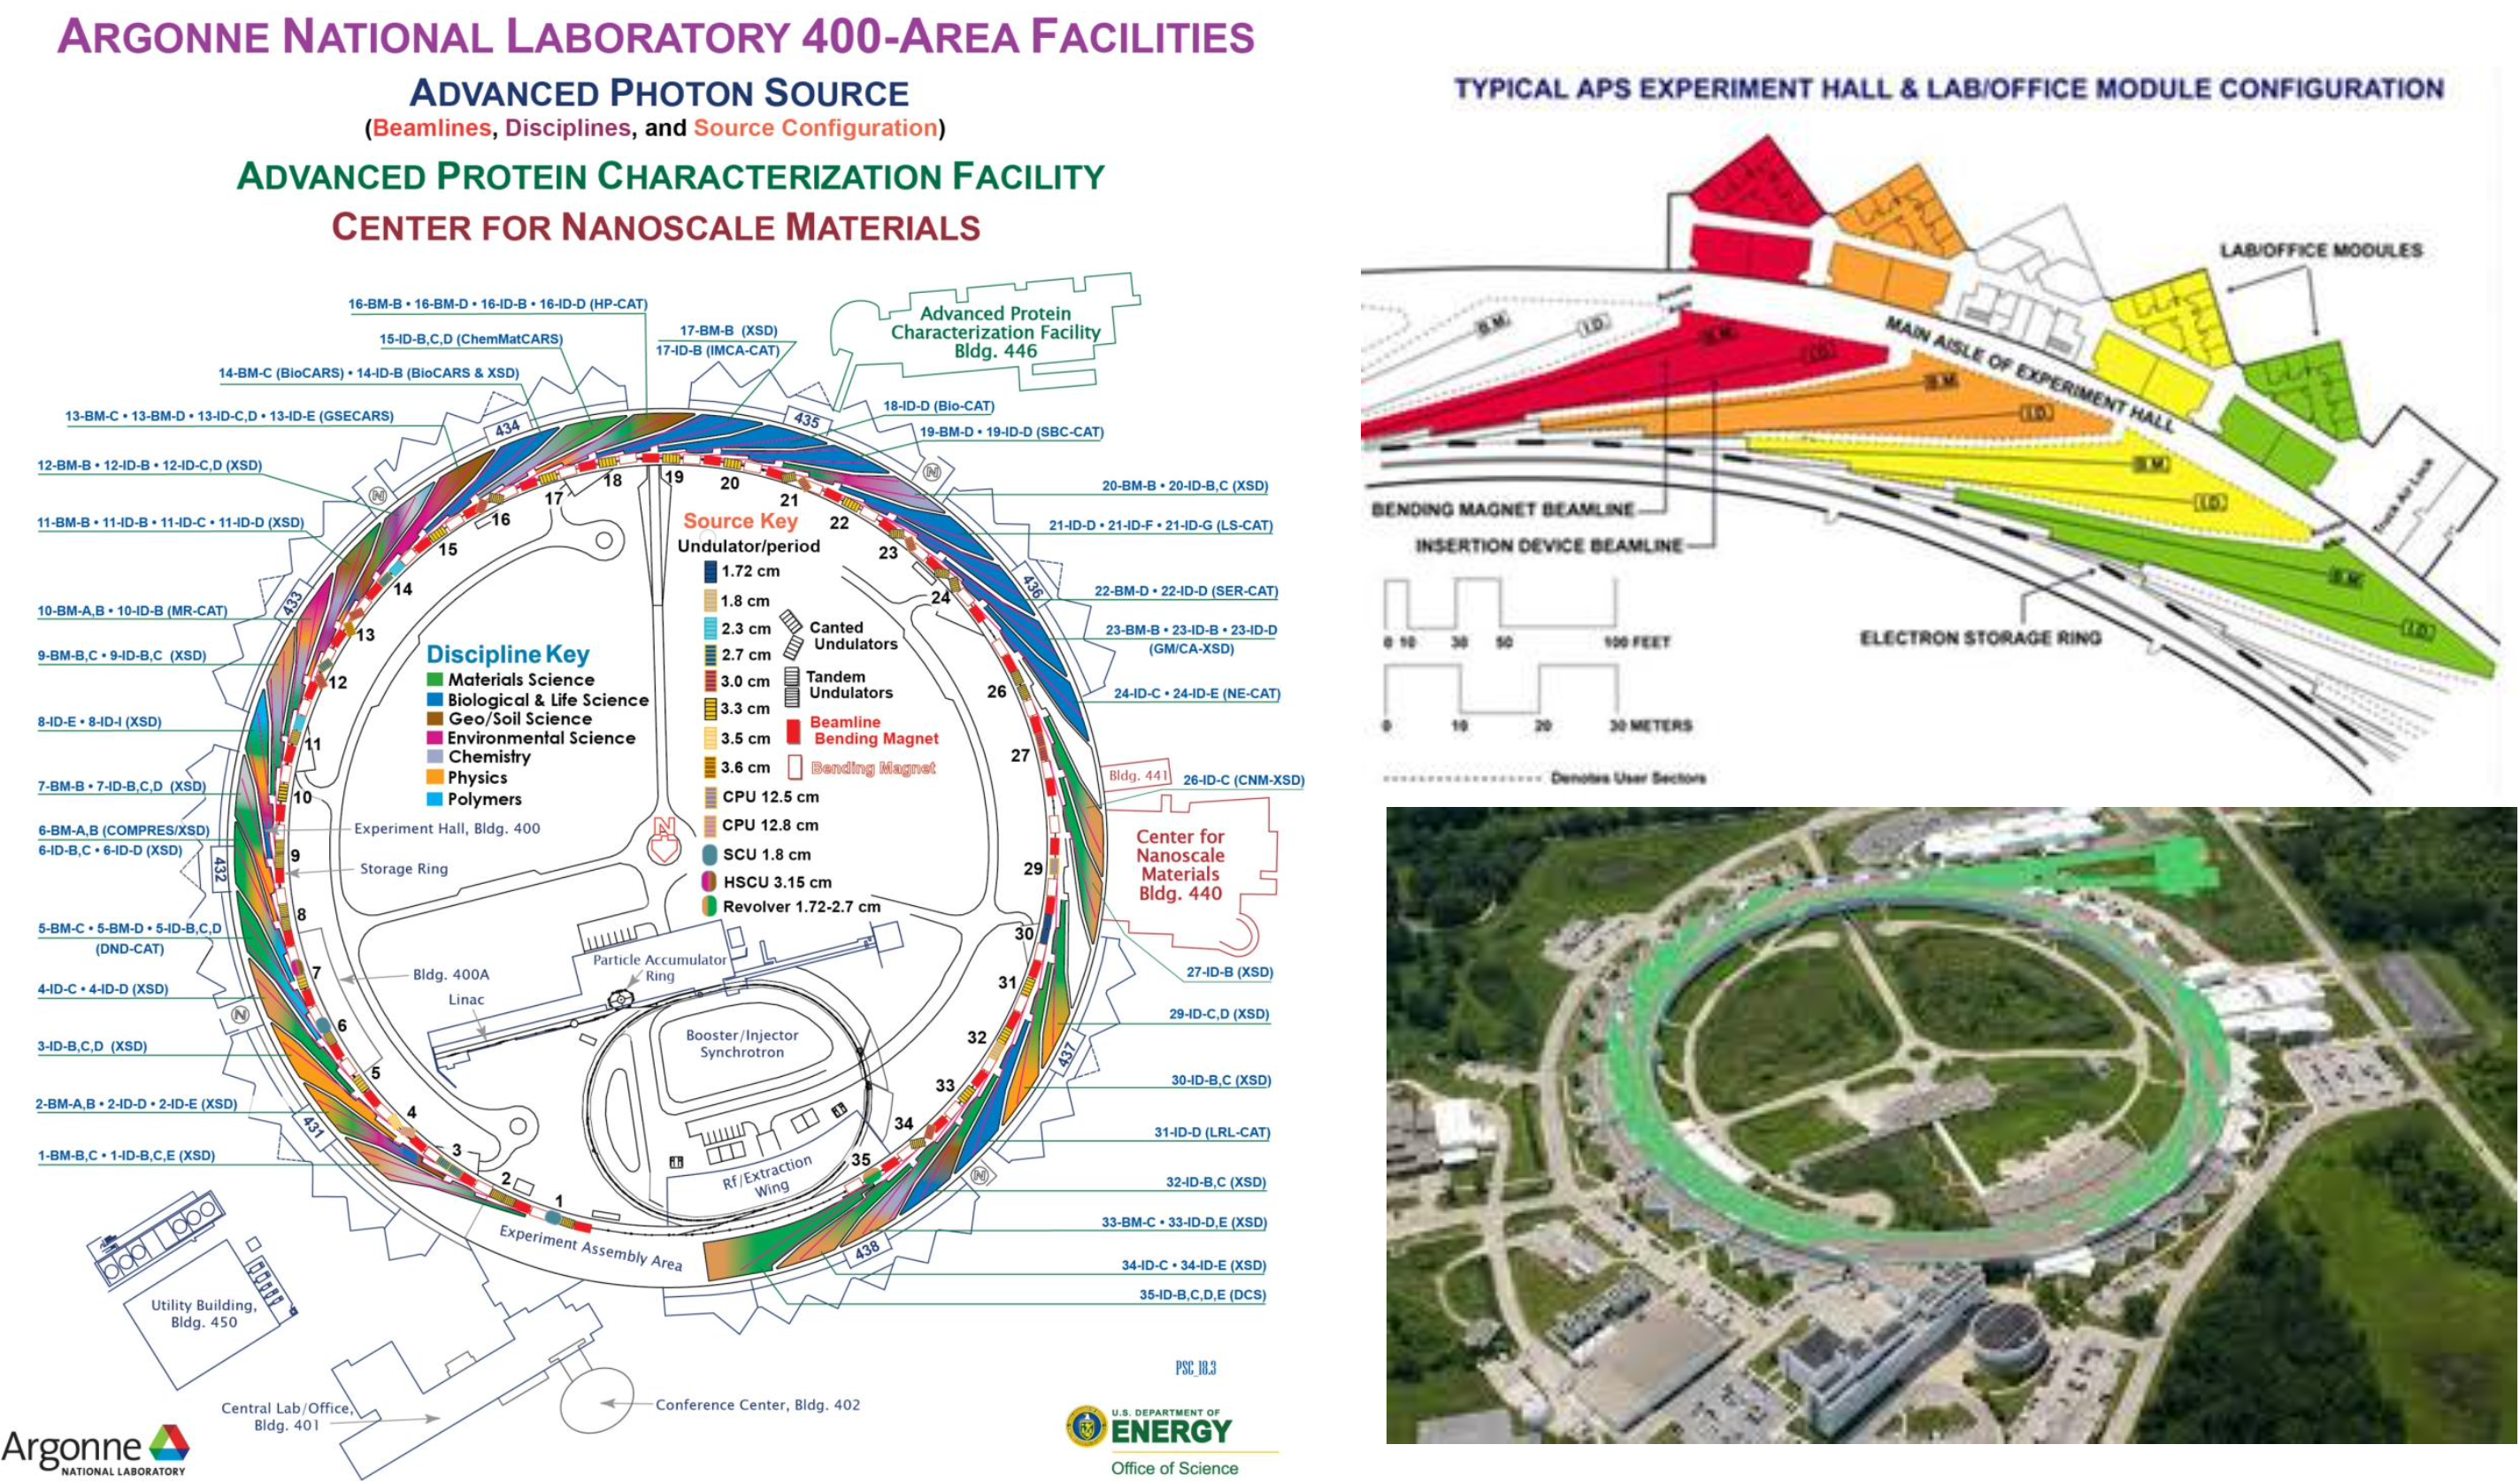
\includegraphics[width=\linewidth]{ArgonneAPS.png}
        \caption{APS at Argonne.}
        \label{fig:ArgonneAPS}
    \end{figure}
    \begin{itemize}
        \item It's a relatively large circular building.
        \item Different numbers correspond to the sectors; each sector has different beamlines.
        \item Along the ring, electrons are traveling.
        \item Electrons are generated in the same way that they're generated in electron microscopes. Then there is an inner circle in which they are traveling. Then they are extracted using magnets and go to the larger circle.
        \item The quality of synchrotron facilities is determined by a few parameters. One of them is the uniformity of the X-rays.
    \end{itemize}
    \item Uniformity of the X-rays.
    \begin{figure}[h!]
        \centering
        \begin{subfigure}[b]{0.33\linewidth}
            \centering
            \includegraphics[width=0.85\linewidth]{uniformXraysa.png}
            \caption{X-ray tube.}
            \label{fig:uniformXraysa}
        \end{subfigure}
        \begin{subfigure}[b]{0.32\linewidth}
            \centering
            \includegraphics[width=0.9\linewidth]{uniformXraysb.png}
            \caption{Bending magnet.}
            \label{fig:uniformXraysb}
        \end{subfigure}
        \begin{subfigure}[b]{0.33\linewidth}
            \centering
            \includegraphics[width=0.9\linewidth]{uniformXraysc.png}
            \caption{Wiggler.}
            \label{fig:uniformXraysc}
        \end{subfigure}\\[2em]
        \begin{subfigure}[b]{0.33\linewidth}
            \centering
            \includegraphics[width=0.9\linewidth]{uniformXraysd.png}
            \caption{Undulator.}
            \label{fig:uniformXraysd}
        \end{subfigure}
        \begin{subfigure}[b]{0.33\linewidth}
            \centering
            \includegraphics[width=0.9\linewidth]{uniformXrayse.png}
            \caption{Free electron laser.}
            \label{fig:uniformXrayse}
        \end{subfigure}
        \caption{Making uniform X-rays.}
        \label{fig:uniformXrays}
    \end{figure}
    \begin{itemize}
        \item Methods of achieving uniform, collimated X-rays.
        \begin{itemize}
            \item Bending magnets (BMs).
            \begin{itemize}
                \item Aren't super precise.
            \end{itemize}
            \item Insertion devices (IDs).
            \begin{itemize}
                \item E.g., \textbf{wigglers} and \textbf{undulators}.
            \end{itemize}
            \item Free electron lasers.
            \item See Figure \ref{fig:uniformXrays} for schematics of all of these.
        \end{itemize}
        \item Look for BMs and IDs in Figure \ref{fig:ArgonneAPS}.
        \item Dipole magnets are used to get \textbf{bends} in the \textbf{design trajectory} (or \textbf{orbit}) of the particles.
        \begin{itemize}
            \item This is what the APS currently uses.
        \end{itemize}
        \item The wavelength of the radiation emitted can be readily tuned by adjusting the energy of the electron beam or the magnetic-field strength.
    \end{itemize}
    \item Undulator/Wiggler I.
    \begin{figure}[h!]
        \centering
        \includegraphics[width=0.5\linewidth]{undulatorWiggler.png}
        \caption{Undulator/wiggler structure.}
        \label{fig:undulatorWiggler}
    \end{figure}
    \begin{itemize}
        \item Undulators/wigglers are insertion devices consisting of a periodic structure of dipole magnets.
        \item History.
        \begin{itemize}
            \item Vitali Ginsburg (1947): Theoretical prediction of undulators.
            \item Hanz Motz (Stanford, 1952): First experimental use to get coherent radiation (IR waves).
        \end{itemize}
        \item The magnets can be permanent or superconducting.
        \begin{itemize}
            \item Synchrotrons use the latter.
        \end{itemize}
        \item The static magnetic field alternates along the length of the undulator with a wavelength $\lambda_u$.
        \begin{itemize}
            \item So we use super small magnets?? How do we get significant enough changes in the magnetic field??
        \end{itemize}
        \item Electrons going through the periodic magnet structure are forced to oscillate, emitting radiation.
        \item The direction of the beam is called the \textbf{longitudinal direction}.
        \item The direction of the beam path is called \textbf{transverse}.
        \item Electromagnetic Lorentz force from the magnetic field causes the electrons in the beam to wiggle transversely.
    \end{itemize}
    \item Undulator/Wiggler II.
    \begin{itemize}
        \item Undulator and wiggler are similar (can be the same device): By increasing or decreasing magnetic field strength or moving permanent magnets closer or farther apart, the device can be setup as a wiggler or undulator.
        \item Determining if a device is an undulator or a wiggler:
        \begin{equation*}
            K = \frac{eB\lambda_u}{2\pi m_ec}
        \end{equation*}
        \item Variable definitions.
        \begin{itemize}
            \item $K$ is an undulator strength parameter (characterizes the nature of electron motion).
            \item $e$ is the electron charge.
            \item $B$ is the magnetic field.
            \item $\lambda_u$ is the spatial period of the undulator magnets.
            \item $m_e$ is the electron rest mass.
            \item $c$ is the speed of light.
        \end{itemize}
        \item We cannot change $e,m_e,c$.
        \item If $K\leq 1$, the oscillation amplitude of the electron motion is small and we get a narrow energy distribution of X-rays.
        \begin{itemize}
            \item The radiation produced is very intense, concentrated in narrow energy bands in the spectrum, and collimated.
            \item This yields an undulator.
        \end{itemize}
        \item If $K\geq 1$, then the oscillation amplitude of the electron motion is big.
        \begin{itemize}
            \item The radiation produced lies in a broad energy distribution of X-rays.
            \item This yields a wiggler.
        \end{itemize}
    \end{itemize}
    \item APS.
    \begin{itemize}
        \item 35 sectors with 68 beamlines (22 BM and 46 undulators; no FEL).
    \end{itemize}
    \item APS upgrade timeline.
    \begin{itemize}
        \item Starts April 17, 2023.
        \item Ends April 2024.
        \begin{itemize}
            \item A similar upgrade at the Advanced Light Source (ALS) at the Lawrence Berkeley National Laboratory is scheduled to begin in 2025.
        \end{itemize}
        \item Shevchenko predicts most of us will get a chance to experience it before it closes.
        \begin{itemize}
            \item I should ask Yingjie about this!
        \end{itemize}
    \end{itemize}
    \item APS upgrade details.
    \begin{itemize}
        \item Upgrade of the storage ring to a Multi-Bend Achromat (MBA) lattice (APS-U).
        \begin{itemize}
            \item Will lead to dramatic improvements in the brightness of the X-rays in both ID and BM beamlines at the APS.
        \end{itemize}
        \item More on the major changes to the storage ring.
        \begin{itemize}
            \item The number of photons will remain the same, but electrons will be really concentrated.
            \item The energy of the electrons will be lowered from 7 to \SI{6}{\giga\electronvolt}.
        \end{itemize}
        \item Don't just memorize this info, but also think about why these changes are needed.
        \begin{itemize}
            \item For example, lowering the energy is necessary because it easier to keep the electrons in the ring (think $mv^2/r$); if we didn't lower energy, we'd need either a whole new facility with a larger radius or stronger magnets (but neither of these are really reasonable).
        \end{itemize}
        \item Major changes to the beamlines.
        \begin{itemize}
            \item New optimized undulators for all the beamlines (ID lines) since the energy of the electrons is changing.
            \item Possibly some BM upgrades?
        \end{itemize}
        \item Reduction of the horizontal emittance of the machine by a factor of about 40 (the number may actually be much higher).
        \begin{itemize}
            \item Leads to a much smaller electron beam source size.
        \end{itemize}
    \end{itemize}
    \item Free-electron laser.
    \begin{itemize}
        \item The principle is the same as for the undulator/wiggler: Indeed, the beam passes through a periodic arrangement of magnets with alternating poles across the beam pass.
        \begin{itemize}
            \item However, the beam of electrons (a lot of them) is accelerated to almost the speed of light (thus, these facilities are huge).
        \end{itemize}
        \item The released photons from an undulator are monochromatic but still incoherent because the electromagnetic waves from randomly distributed electrons can interfere constructively and destructively.
        \begin{itemize}
            \item To solve this problem, FELs send electrons in a bunch --- the radiation emitted by the bunched electrons can be in phase and hence is coherent.
            \item Implies great time resolution (useful for studying \ce{CdSe}, etc. by sending pulses).
        \end{itemize}
        \item The credit for these machines should be given to John Madley (Stanford, 1971). He built on Motz's work on the undulator.
        \item The released photons are captured by mirrors in the laser cavity, inducing more electrons to emit light, resulting in amplification of the light.
        \item It is very difficult to get time at these facilities.
    \end{itemize}
    \item We now talk about some examples of high-pressure studies at APS.
    \item Diamond anvil cell program at GSECARRs (Sector 13).
    \begin{itemize}
        \item Raman, infrared, visible, XRD, heat, etc. All kinds!
        \item If you're planning an experiment, talk to someone at the beamline.
        \item I should read that XAFS basics book more!
    \end{itemize}
    \item A few examples will be wrapped up next time.
\end{itemize}



\section{Office Hours (Shevchenko)}
\begin{itemize}
    \item \marginnote{1/13:}What do you want us to know about MXenes, esp. concerning variable termination groups?
    \begin{itemize}
        \item There may be questions about these on the exams.
        \item Very popular; worth Googling. One of the hottest materials in material science right now. Used for everything.
        \item You take a MAX phase and etch aluminum out of it.
        \item Termination: You start with a MAX phase, then using \ce{HF} or some other mixture that generates it (e.g., \ce{LiF}, \ce{HCl}), you will etch aluminum and get these.
        \item You can use molten salts for synthesis and termination of MXenes.
        \item Worth introducing these materials as examples of things we can characterize.
        \item Suppose we study these with XRD; how will certain peaks change/disappear?
        \item Metal, carbon, aluminum. You remove the aluminum.
        \item MAX phase (metal, aluminum, X for something else [carbon or nitride]).
        \item A bunch of layers that are glued together with aluminum; you remove the aluminum with acid etching, yielding free-standing layers that are several atoms thick. T stands for termination. Either \ce{OH} or \ce{=O} groups.
        \item Synthesis can be scaled up; this is why they're popular.
        \item Solution at the bottom shows that you can scale it up.
        \item The layers can interact via van der Waals interactions and stay together. When you do microscopy, the samples can be oriented differently.
        \item Lithium can intercalate into these materials.
        \item As MXenes separate, fewer peaks in the small $2\theta$ area (corresponding to big interplanar distances).
        \item Don't need to know anything about the synthesis of the MAX phase; just assume it exists.
        \item Different functional capping groups are useful when you want to change the functionality. OH is hard to replace; others may be easier to substitute out.
        \item You can use molten salts to do etching in addition to acid; hot metal ions diffuse into the layers and remove aluminum.
        \item Talapin and another guy at Drexel are very strong in MXenes. Even as a generic chemist, I will probably overlap with this type of material at some point!
    \end{itemize}
    \item With respect to an X-ray tube, you said that reducing the tube current to \SI{100}{\milli\ampere} from \SI{200}{\milli\ampere} increases the lifetime by 50\%. Are there drawbacks to doing this or any real reason not to?
    \begin{itemize}
        \item Not information worth remembering.
        \item Instruments are built to only last so long so companies don't have to do back compatibility.
    \end{itemize}
    \item Bremsstrahlung radiation: You called it "inelastic scattering." How? Because energy is lost to radiation?
    \item Bremsstrahlung radiation: How does an increase in peak intensity result from an increase in energy of the particle to be decelerated? Is it because these higher energy particles more readily give off energy?
    \item \ce{Fe}, \ce{Cr}, and \ce{Mn} fluoresce under the \ce{Cu} $K_\alpha$ beam. To mitigate this effect, is it that we want to switch to an instrument that doesn't use \ce{Cu} or \ce{Co}, or switch from one that uses \ce{Cu} to one that uses \ce{Co}.
    \begin{itemize}
        \item Switching to cobalt can work. You just have to make sure that the concerning elements don't fluoresce under the new radiation. Unless you're in a specialized lab, though, you won't have both a copper and cobalt instrument in the same lab. Cobalt is mainly used in older instruments. Best solution: Use a syncrotron, because there you can adjust the energy of electrons.
    \end{itemize}
    \item Working principle of a monochromator: Can't we just orient it at the angle we need to select for the wavelength we want for any suitably crystalline material? Check the derivation.
    \begin{itemize}
        \item We do have to align the monochromator correctly.
    \end{itemize}
    \item Divergence slits vs. beam masks?
    \begin{itemize}
        \item Divergence slits and masks refine the beam in different ways (vertical vs. horizontal).
        \item Controls what's illuminated.
        \item Shevchenko is not quite sure why we would want to do this.
        \item Better than a hole just because it's easier to control.
        \item You can insert these things partially.
    \end{itemize}
    \item What are 0D, 1D, and 2D detectors?
    \begin{itemize}
        \item Signals get generated in every direction when your beam impinges on the sample; this just determines how many points you observe.
        \item For APS, 0D and 1D are functionally the same.
        \item 2D allows you to get the whole picture right away.
        \item Allows us to improve the resolution of the signal if we have higher dimensions.
        \item There may not be much difference though.
        \item Important because companies always specify which they're machines are, so it's good to understand it.
        \item Detector type may not be tied to geometry.
    \end{itemize}
    \item Takeaways from your discussion of grazing incidence XRD?
    \begin{itemize}
        \item The two detectors move at the same pace in both, but there is a fixed offset angle.
        \item Think about the surface of a thin film.
        \item Initial angle is closest to your surface. At smaller angles, you have a higher chance of interacting with the thin film. Side of a piece of paper visual.
        \item We don't go to all the angles, just the low ones.
        \item Read more about this online.
        \item We use this to study the surface.
    \end{itemize}
    \item Clarification on primitive vs. non-primitive unit cells?
    \item Notation: Set of all parallel vectors pointing in the direction $(4,-2)$ should be denoted $<4\bar{2}>$?
    \item Reading space groups: Glide planes?
    \item To confirm, in a space group, three symmetry elements can describe the full symmetry?
    \item Space groups: Viewing directions for different Bravais lattices. What do we need to know?
    \begin{itemize}
        \item We don't need to pay much attention to space groups.
        \item Important for very careful analyses, new materials that need proper characterization, etc. But not important for common use.
        \item Very simple questinos about this only, needig common knowledge
    \end{itemize}
    \item What is $L$?
    \begin{itemize}
        \item Just generic.
    \end{itemize}
    \item How much do you expect we know about XRD coming in?
    \begin{itemize}
        \item Closer to the exam, Shevchenko will say which questions on the midterm will cover which topics (this, that, or that)?
        \item This is a grad-student course, so you know symmetry groups and stuff but not much about XRD.
        \item One explanation will give you full credit for things when multiple factor could be relevant.
        \begin{itemize}
            \item For example, if you observe a shift in peak positions, you could talk about compression for instance.
            \item As long as you're close enough, full credit.
            \item What kind of media do use for higher compression in DACs, or what is the best pressure-transmitting medium?
        \end{itemize}
        \item It will be open note.
        \item Last time, one student did fantastic, most did very well, and 2 struggled.
    \end{itemize}
\end{itemize}




\end{document}